\documentclass[../../main.tex]{subfiles}
\graphicspath{{../../image/}{../../figure/}}
\begin{document}

\section{激波与凸壁的碰撞}\label{section:ch18-激波撞凸壁}

在状态方程为\eqref{align:ch18-18317}的理想气体二维势流范围内，此处考察激波与固体凸壁的碰撞。在 $x$-$y$ 平面的上半平面，凸壁根部位于原点，斜率为 $\tan\omega$。激波平行于 $y$ 轴，自左向右运动，在零时刻位于 $y$ 轴上。在其左侧 $x<0$，气体具有常密度 $\rho_f$ 与常速度 $(u_f,0)$，$u_f>0$。在其右侧 $x>0$、凸壁上方，气体具有常密度 $\rho_d$，$\rho_d<\rho_f$，并处于静止，即 $u_d=v_d=0$。等价地，可把这一构型看作激波与楔碰撞（顶点角为 $2\omega$）的上半部分。

于是寻求某势流 $(\rho,u,v)$，定义在区域 $\{(x,y):x<0,\ 0\leqslant y<\infty\}\cup\{(x,y):x\geqslant0,\ x\tan\omega\leqslant y<\infty\}$ 上，并满足边界条件
\begin{align}
v(x,0,t)=0,\qquad -\infty<x<0,\ 0<t<\infty,
\label{align:ch18-1861}
\end{align}
\begin{align}
v(x,x\tan\omega,t)=u(x,x\tan\omega,t)\tan\omega,\qquad 0\leqslant x<\infty,\ 0<t<\infty,
\label{align:ch18-1862}
\end{align}
以及初始条件
\begin{align}
(\rho,u,v)(x,y,0)=
\begin{cases}
(\rho_f,u_f,0), & -\infty<x<0,\ 0\leqslant y<\infty\\
(\rho_d,0,0), & 0\leqslant x<\infty,\ x\tan\omega\leqslant y<\infty,
\end{cases}
\label{align:ch18-1863}
\end{align}
其中状态 $(\rho_f,u_f,0)$ 与 $(\rho_d,0,0)$，$u_f>0$，$\rho_f>\rho_d$，由一道可容激波连接。

由于区域几何与数据的伸缩不变性，上述问题的解是自相似的，即 $\rho,u,v$ 与伪势 $\chi$ 可实现为两个变量 $\xi=x/t$、$\zeta=y/t$ 在区域 $\{(\xi,\zeta):\xi<0,\ 0\leqslant\zeta<\infty\}\cup\{(\xi,\zeta):\xi\geqslant0,\ \xi\tan\omega\leqslant\zeta<\infty\}$ 上的函数。

\begin{figure}[ht]
\centering
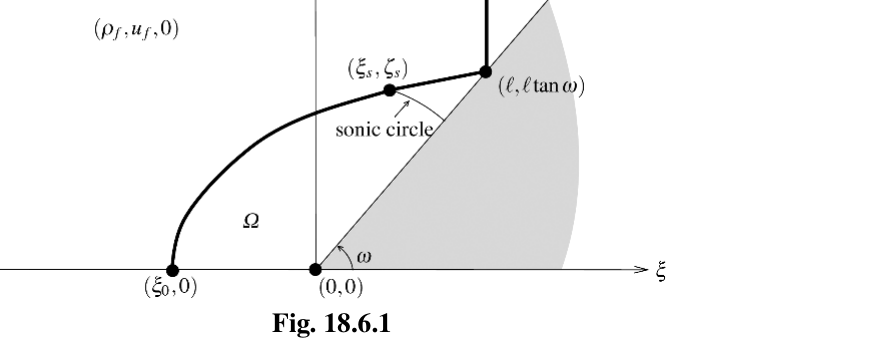
\includegraphics[width=0.85\textwidth]{ch18-fig06-01.png}
\caption{激波与凸壁碰撞：入射激波在 $(\ell,\ell\tan\omega)$ 处正规反射，反射激波在 $(\xi_s,\zeta_s)$ 处穿过声速圆后被衍射，垂直地击中 $\xi$ 轴于 $(\xi_0,0)$。区域 $\Omega$ 为亚声速。}
\label{figure:ch18-激波撞壁}
\end{figure}

在 $\xi$-$\zeta$ 平面上，入射激波将在点 $(\ell,\ell\tan\omega)$ 与凸壁接触。在该点附近，凸壁根部（$\xi<0$）左侧的边界条件不会影响解。因而，在 $\omega>\omega_d$ 的假设下，其中 $\omega_d$ 是\cref{section:ch18-正规激波反射}中确定的脱体角，入射激波将在 $(\ell,\ell\tan\omega)$ 处发生正规反射。特别地，$\ell$ 以及 $\rho_f,u_f$ 与 $\rho_d$ 之间的必要关系仍通过\eqref{align:ch18-1851}与\eqref{align:ch18-1853}确定。反射激波从 $(\ell,\ell\tan\omega)$ 发出，斜率为 $\tan\theta$，连接前面状态 $(\rho_f,u_f,0)$ 与后状态 $(\rho_b,u_b,v_b)$，后者通过\eqref{align:ch18-18510}、\eqref{align:ch18-18511}与\eqref{align:ch18-18512}确定。

设 $\omega>\omega_s$，其中 $\omega_s$ 是\cref{section:ch18-正规激波反射}中确定的声速角。则点 $(\ell,\ell\tan\omega)$ 位于状态 $(\rho_b,u_b,v_b)$ 的声速圆之外，该圆以凸壁上的点 $(u_b,v_b)$ 为圆心，半径 $c(\rho_b)=\sqrt{\gamma-1}\,\rho_b^{\frac{\gamma-1}{2}}$。于是起初反射激波是超声速的，并保持其常斜率，直到它穿入上述声速圆。此外，左侧以声速圆为界、上方以反射激波为界、下方以凸壁为界的区域，是常状态 $(\rho_b,u_b,v_b)$。

解的常状态上的伪势 $\chi$ 由\eqref{align:ch18-1839}确定，常数的选取应保证跨过激波连续。于是，在常状态 $(\rho_d,0,0)$ 上，
\begin{align}
\chi=-\frac12(\xi^2+\zeta^2),
\label{align:ch18-1864}
\end{align}
在常状态 $(\rho_f,u_f,0)$ 上，
\begin{align}
\chi=u_f(\xi-\ell)-\frac12(\xi^2+\zeta^2),
\label{align:ch18-1865}
\end{align}
在常状态 $(\rho_b,u_b,v_b)$ 上，
\begin{align}
\chi=u_b\xi+v_b\zeta-\frac12(\xi^2+\zeta^2)-\frac{1+\tan^2\omega}{1+\tan\omega\tan\theta}\ell u_f.
\label{align:ch18-1866}
\end{align}

在点 $(\xi_s,\zeta_s)$ 处穿过 $(\rho_b,u_b,v_b)$ 的声速圆后，反射激波发生衍射，因为它受到边界条件 $v(\xi,0)=0$（$\xi<0$）的影响，这使其变为凹的。可以证明：若 $u_f\leqslant c(\rho_f)$（如入射激波相对较弱时的情形），衍射激波最终在点 $(\xi_0,0)$，$\xi_0<0$，处以直角击中 $\xi$ 轴，如图\cref{figure:ch18-激波撞壁}所示。为验证这一构型并完成流动构造，须在图\cref{figure:ch18-激波撞壁}中标为 $\Omega$ 的区域内确定伪势 $\chi$，该区域下方以半坐标轴 $\xi<0$ 与凸壁为界，上方以反射激波与 $(\rho_b,u_b,v_b)$ 的声速圆为界。这通过在 $\Omega$ 上求解椭圆型偏微分方程\eqref{align:ch18-18415}实现，边界条件如下：沿底部边界段，由\eqref{align:ch18-1861}与\eqref{align:ch18-1862}要求 $\partial\chi/\partial\nu=0$。沿声速圆弧，取 $\chi_\xi=u_d-\xi$、$\chi_\zeta=v_d-\zeta$，以保证速度场跨过该曲线连续。最后，跳跃条件\eqref{align:ch18-18315}与\eqref{align:ch18-18316}必须跨过激波成立。这一问题展现出\cref{section:ch18-超声速绕凸角}中已遇到的困难：第一，跨声速激波的图像事先未知，它是一个须作为解的一部分来确定的自由边界；第二，在声速圆上同时给定了 Dirichlet 与 Neuman 数据，而椭圆性恰在那里退化。克服这些障碍所需的艰苦技术性分析超出本书范围，载于\cref{section:ch18-注记}所引文献。结论综述如下。

\begin{theorem}[激波绕凸壁的衍射]\label{theorem:ch18-激波绕凸壁衍射}
在假设 $\omega>\omega_s$ 且 $u_f\leqslant c(\rho_f)$ 下，存在一分段光滑、自相似的势流 $(\rho,u,v)$，满足边界条件\eqref{align:ch18-1861}、\eqref{align:ch18-1862}与初始条件\eqref{align:ch18-1863}。其构型如图\cref{figure:ch18-激波撞壁}所示，具有如下特征：
\begin{enumerate}
\item\label{item:ch18-衍射-a} 连接 $(\rho_f,u_f,0)$ 与 $(\rho_d,0,0)$ 的入射激波，在凸壁上的点 $(\ell,\ell\tan\omega)$ 处发生正规反射。
\item\label{item:ch18-衍射-b} 反射激波 $\zeta=\sigma(\xi)$ 从 $(\ell,\ell\tan\omega)$ 发出，终止于 $\xi$ 轴上的点 $(\xi_0,0)$。它在 $\xi_0<\xi<\ell$ 段是超声速的，$\sigma(\xi)=\ell\tan\omega+(\xi-\ell)\tan\theta$，连接 $(\rho_f,u_f,0)$ 与 $(\rho_b,u_b,v_b)$；在 $\xi_0<\xi<\xi_s$ 段跨声速。此外，$\sigma$ 在 $\xi_s$ 处为 $C^2$，在 $(\xi_0,\xi_s)$ 上为 $C^\infty$。
\item\label{item:ch18-衍射-c} 入射激波前方的区域是常状态 $(\rho_d,0,0)$。
\item\label{item:ch18-衍射-d} 入射激波后方、反射激波前方的区域是常状态 $(\rho_f,u_f,0)$。
\item\label{item:ch18-衍射-e} 反射激波超声速部分后方、位于 $(\rho_b,u_b,v_b)$ 的声速圆之外的区域，是常状态 $(\rho_b,u_b,v_b)$。
\item\label{item:ch18-衍射-f} 在反射激波跨声速部分后方、右以 $(\rho_b,u_b,v_b)$ 的声速圆为界的区域 $\Omega$ 内，$(\rho,u,v)$ 是 $C^\infty$ 的，$(u,v)$ 由 $C^\infty$ 伪势 $\chi$ 导出，$\chi$ 满足椭圆方程\eqref{align:ch18-18415}。
\item\label{item:ch18-衍射-g} $(\rho,u,v)$ 跨过分界 $\Omega$ 的 $(\rho_b,u_b,v_b)$ 的声速圆弧时是 Lipschitz 的。
\end{enumerate}
\end{theorem}

假设 $\omega>\omega_s$ 与 $u_f\leqslant c(\rho_f)$ 中一个或两个被违反的情形，在\cref{section:ch18-注记}所引文献中讨论。结果表明：当 $\omega\in[\omega_d,\omega_s]$ 但仍有 $u_f\leqslant c(\rho_f)$ 时，在点 $(\ell,\ell\tan\omega)$ 处的反射变为跨声速，最终得到与图\cref{figure:ch18-激波撞壁}相同的构型，只是此时点 $(\xi_s,\zeta_s)$ 与 $(\ell,\ell\tan\omega)$ 重合，反射激波全程保持跨声速；而整个区域 $\Omega$（下方以半坐标轴 $\xi<0$ 与凸壁为界，上方以反射激波为界）是亚声速的。

当 $u_f>c(\rho_f)$ 时，上述描述仍成立，但只在 $\omega$ 超过某临界角 $\omega_c\in[\omega_d,\frac12\pi)$ 时。当 $\omega$ 趋近 $\omega_c$ 时，图\cref{figure:ch18-激波撞壁}中的点 $(\xi_0,0)$ 向原点 $(0,0)$ 靠近，并在 $\omega=\omega_c$ 时与之合并，此时反射激波附着于凸壁根部。

\end{document}
